%----------------------------------------------------------------------------------------------------------------
\chapter[初步结果]{初步结果}
\label{chap3}
\section{toy model测试结果}
下面通过两个数值例子介绍PPSDNN的算法实现以及一些更多的算法细节。第一个数值的例子是训练一个有确定函数形式生成的数据,且我们可以根据它的函数形式大致确定其频域空间的范围,在第一个例子中将引入和PPSDNN等价的另一种实现phase shift的方法。
第二个数值例子是训练一个不光滑的函数生成的数据,它的特点是根据函数形式无法大致确定其频域空间的范围,因此在第二个例子中引入频率扫荡方法(frequency sweep)。此外,PPSDNN还可以用来拟合多维的振荡数据,解高频的波动方程,亥姆霍兹方程等,但这些应用不在本文的范围之内。

首先介绍第一个数值例子。在第一个例子中,我们选取目标函数f(x)的定义域为$[-\pi,\pi]$,函数形式为
\begin{equation}\label{eq:target1}
    f(x) = \begin{cases}
             10(\sin x + \sin 3x), & \mbox{如果 } x\in [-\pi,0] \\
             10(\sin 23x + \sin 137x + \sin 203x), & \mbox{如果 }x\in [0,\pi].
           \end{cases}
  \end{equation}
在定义域上画出函数图形,如图\ref{toy}所示。
\begin{figure}[htbp]
  \centering
  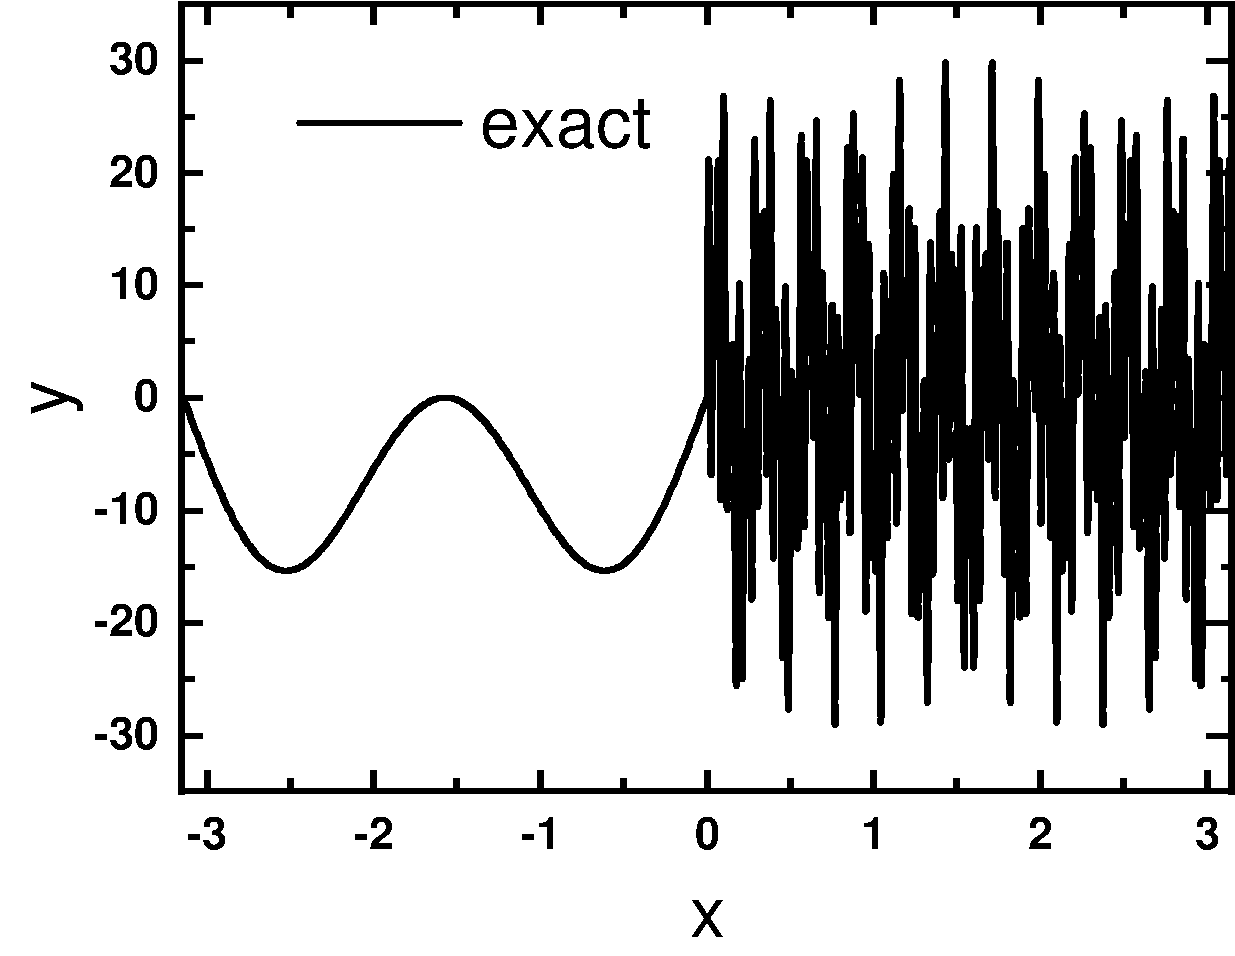
\includegraphics[width=0.76\linewidth]{figures/toymodel/exact.pdf}
  \caption{toy model目标函数\ref{eq:target1}式的图形}
  \label{toy}
\end{figure}

  因为该函数的频率空间可以从它的函数形式或通过傅里叶变换得到,因此我们取$\Delta k=5$,用以下的特征函数对目标函数进行单位分解。
  \begin{equation}\label{}
    \begin{aligned}
      &\phi_1(k) = \chi_{[-205,-200]}(k)  & \phi_2(k) = \chi_{[-140,-135]}(k)\\
      & \phi_3(k) = \chi_{[-25,-20]}(k)  & \phi_4(k) = \chi_{[-5,0]}(k)\\
      &\phi_5(k) = \chi_{[0,5]}(k)   & \phi_6(k) = \chi_{[20,25]}(k)\\
      & \phi_7(k) = \chi_{[135,140]}(k)  & \phi_8(k) = \chi_{[200,205]}(k)
      \end{aligned}
  \end{equation}
  则$f_j(x) = \mathcal{F}^{-1}[\widehat{f}\phi_j](x)$。训练DNN的参数为:
  \begin{itemize}
    \item DNN结构:1-40-40-40-40-1
    \item 训练集:函数定义域上均匀分布的10,000个数据点
    \item 测试集:函数定义域上均匀分布的1000个数据点
    \item epochs:1000
    \item 优化器:Adam
    \item 学习率:0.002
    \item batchsize:2000
  \end{itemize}

  训练的整体结果结果如图\ref{sin}所示,训练结果在各个区间的细节表现如图\ref{toy1},\ref{toy2},\ref{toy3}所示。
\begin{figure}[htbp!]
  \centering
  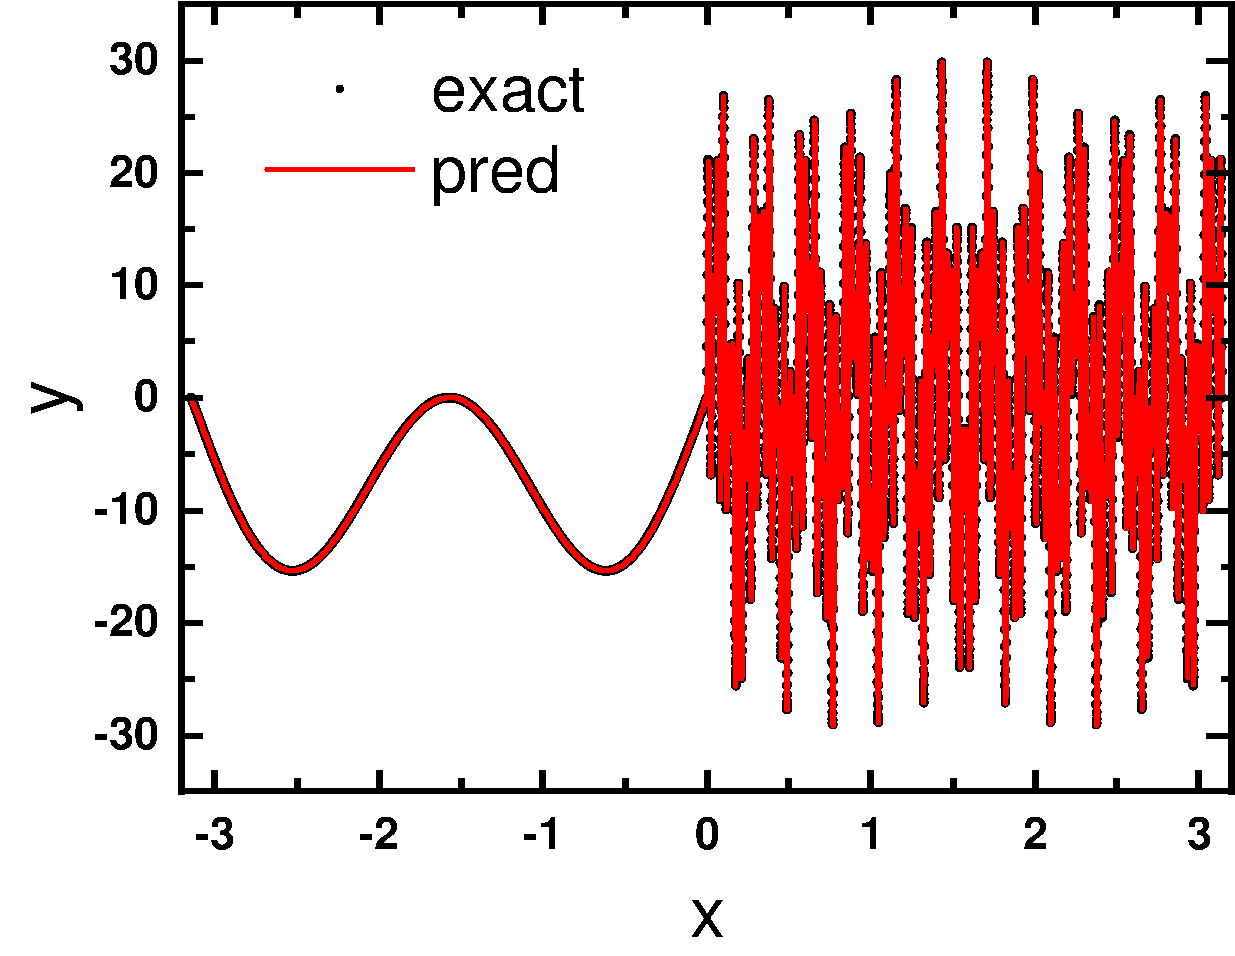
\includegraphics[width=0.77\linewidth]{figures/toymodel/train.pdf}
  \caption{使用PPSDNN训练目标函数\ref{eq:target1}式}
  \label{sin}
\end{figure}
\begin{figure}[htbp]
  \centering
  \includegraphics[width=0.76\linewidth]{figures/toymodel/train1.pdf}
  \caption{toy model在区间$[0,1]$上的训练结果}
  \label{toy1}
\end{figure}
\begin{figure}[htbp]
  \centering
  \includegraphics[width=0.76\linewidth]{figures/toymodel/train2.pdf}
  \caption{toy model在区间$[1,2]$上的训练结果}
  \label{toy2}
\end{figure}
\begin{figure}[htbp]
  \centering
  \includegraphics[width=0.76\linewidth]{figures/toymodel/train3.pdf}
  \caption{toy model在区间$[2,3.14]$上的训练结果}
  \label{toy3}
\end{figure}
  


  在PPSDNN中,由于频率选择核要与训练数据做卷积运算,因此,在高维的卷积运算中,它的空间复杂度为$O (N\times N)$,说明平行相移的方法存在维数灾难,为了避免这个问题,人们提出了Coupled Weighted phase shift DNN\cite{cai2020phase}(CPSDNN):
  \begin{equation} \label{eq:CPDNNcomplex}%
    T(x)=\sum_{m=1}^{M}e^{i\omega_{m}x}T_{m}(x),
    \end{equation}
    其中$\{\omega_{m}\}_{m=1}^M$是和目标函数有关的频率空间。将指数项写成实数的形式为
    \begin{equation}\label{eq:CPDNNreal}%
      T(x)=\sum_{m=1}^{M}A_{m}\cos(\omega_{m}x)+B_{m}\sin(\omega_{m}x),
      \end{equation}
    于是,我们可以定义并最小化损失函数:
    \begin{equation}
      \begin{aligned}
      L(\theta) &= \int_{-\infty}^{+\infty}|f(x)-T(x)|^2d x,\label{eq:2}%
      \end{aligned}
      \end{equation}
      在离散情况下可以写成:
      \begin{equation}
        L_N(\theta) = \sum_{i=1}^{N}\left\vert
        f(x_{i})-T(x_{i})\right\vert ^{2}
        =\sum_{i=1}^{N}\left\vert f(x_{i})-\sum_{m=1}^{M}e^{i\omega_{m}x_{i}}T_{m}(x_{i})\right\vert ^{2}. \label{eq:Ln2}%
        \end{equation}
在实际应用中,我们往往引入正则项,于是损失函数可以改写为
\begin{equation}
  L_N^R(\theta) = \sum_{i=1}^{N}|f(x_i) - T(x_i)|^2 + \beta \sum_{m,l} \norm{\vec{W}^{m, l}}_F^2.
  \end{equation}
  其中,$\beta$是正则化参数,$\vec{W}^{m, l}$是$T_m$的权重矩阵。可以证明,PPSDNN方法和CPSDNN方法训练效果是等价的,而CPSDNN来源于PPSDNN算法的启发。

%   当使用CPSDNN训练第一个例子是,我们选取$\{\omega_{m}\}=\{0,5,25,135,200\}$,其他参数和PPSDNN相同。
%   下面图\ref{1D-10000}是普通DNN方法和CPSDNN方法对第一个数值例子的训练结果比较。
% \begin{figure}[htbp!]
%   \centering
%   \includegraphics[width=0.84\linewidth]{figures/PPSDNN/1D-10000.pdf}
%   \caption{普通DNN和CPSDNN对高频目标函数训练的比较}
%   \label{1D-10000}
% \end{figure}

下面介绍第二个数值例子。在实际工作中,我们学习的核数据一般都是离散的,不像第一个例子生成的函数是连续且光滑的。这时候我们就要用到频率扫荡(frequency sweep)方法。前面取的$\omega _m$都是几个离散的值,在frequency sweep中,我们可以取形如$\omega _m=-1600:10:1600$这样连续的值。我们将\ref{eq:target1}的函数稍作修改,将x小于零的部分改成阶跃函数,使它的频率空间不再那么确定,接着使用frequency sweep进行训练。

训练效果如图\ref{sweep}\cite{cai2019phasednn}所示。
\begin{figure}[htbp!]
  \centering
  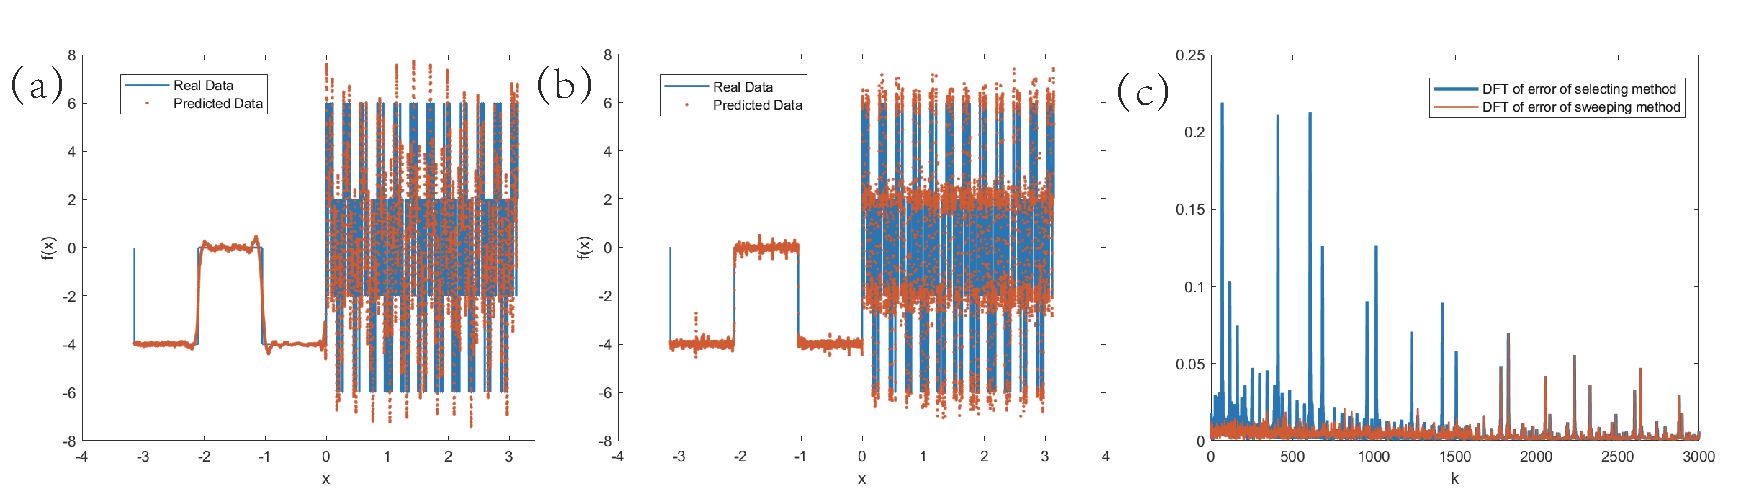
\includegraphics[width=0.84\linewidth]{figures/PPSDNN/1D-square.pdf}
  \caption{使用frequency sweep训练高频函数}
  \label{sweep}
\end{figure}


\section{$^{235}\text{U}(n,f)$评价库数据测试结果}
根据核反应的复合核理论,当中子与靶核形成复合核时,复合核的激发能为
\begin{equation}\label{}
  E^{\ast } = \frac{m_A}{m_n+m_A}E_n+B_{nA}.
\end{equation}
其中,$m_A$为靶核的质量,$m_n$为中子的质量,$E_n$为入射中子的相对动能,$B_{nA}$为中子与靶核的结合能。当形成的复合核能级等于$E^{\ast }$时,入射粒子被强烈吸收,形成共振峰。
% 在此工作中,我们以$^{235}\text{U}(n,f)$反应为例,使用PPSDNN方法,对其截面数据进行学习研究。此反应的实验数据和ENDF/B-VIII.0评价库的数据如图\ref{u235expendf}所示.

近几十年以来,$^{235}\text{U}$中子共振区的实验测量和理论研究一直是生机勃勃的,累计的实验截面数据估计在10万以上。由于测量技术,参数分析方法的不同,共振参数间存在着分歧。同时,一家测量分析的结果往往不能覆盖全部能区和给出全部共振参数。因此,综合多家实验数据进行分析评价是十分必要的\cite{何锦昌1990中子共振参数的联合拟合分析}。而目前最核心的技术难题就是难以拟合好高频振荡的数据。在$\text{n}+^{235}\text{U}$反应中,存在多种截面数据,包括裂变截面,俘获截面,全截面等。本工作研究的是裂变截面。


ENDF/B-VIII.0是美国核反应数据库ENDF的最新版本,于2018年2月2日发布\cite{Brown2018}。它完全采用了新的中子数据标准,改进了热中子散射数据,并使用了国际评价库组织(CIELO)试点项目的新评价数据,涵盖了氢、氧、铁、铀和钚等元素的中子反应\cite{Sobes2021}。由于评价库中的核数据与实验核数据相比,其截面数据的连续性与光滑性更好,因此更适合使用神经网络方法进行学习。
下面将分别使用普通DNN方法和PPSDNN方法学习这些实验数据以及评价库中的数据。



在此部分,首先介绍普通DNN方法在研究$^{235}\text{U}(n,f)$反应中的应用。根据第二章的分析,由于f- principle,DNN方法更偏向于先学习低频数据,再学习高频数据,因此,在中子共振区域,在有限运算资源的情况下,DNN方法的学习效果并不会很好。

由于实验数据每家测量的分歧较大,因此为了快速从实践上验证PPSDNN在中子共振中应用的可行性,本文采用ENDF/B-VIII.0的数据作为学习数据集。
图\ref{endftrain}到图\ref{endf1}是使用PPSDNN方法对$^{235}\text{U}(n,f)$反应的评价库数据进行学习的结果。
% 下面是使用ENDF/B-VIII.0库的学习结果。如图
\begin{figure}[htbp!]
  \centering
  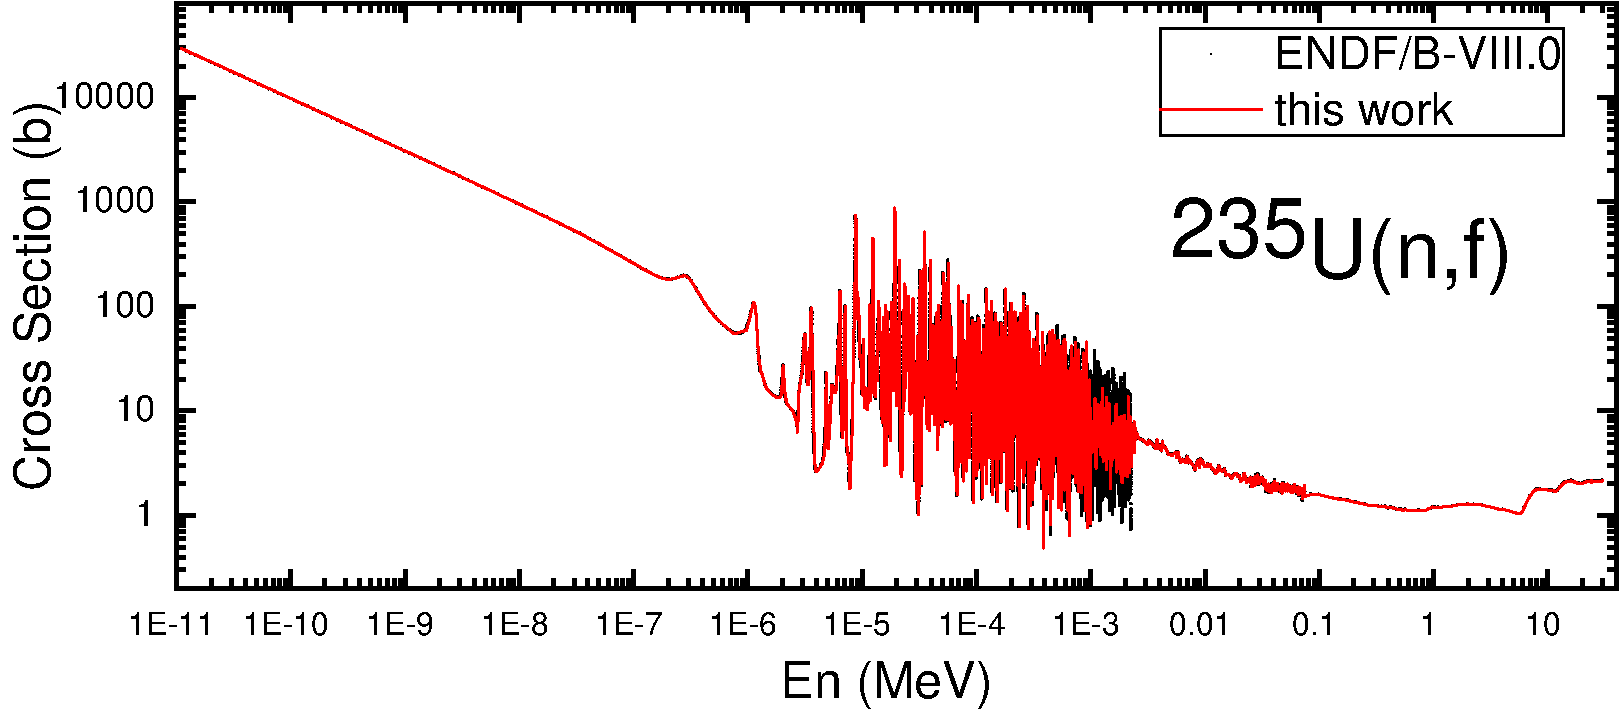
\includegraphics[width=0.94\linewidth]{figures/endftrain/endftrain.pdf}
  \caption{PPSDNN方法对ENDF/B-VIII.0数据库中$^{235}\text{U}(n,f)$反应截面的学习}
  \label{endftrain}
\end{figure}
\begin{figure}[htbp!]
  \centering
  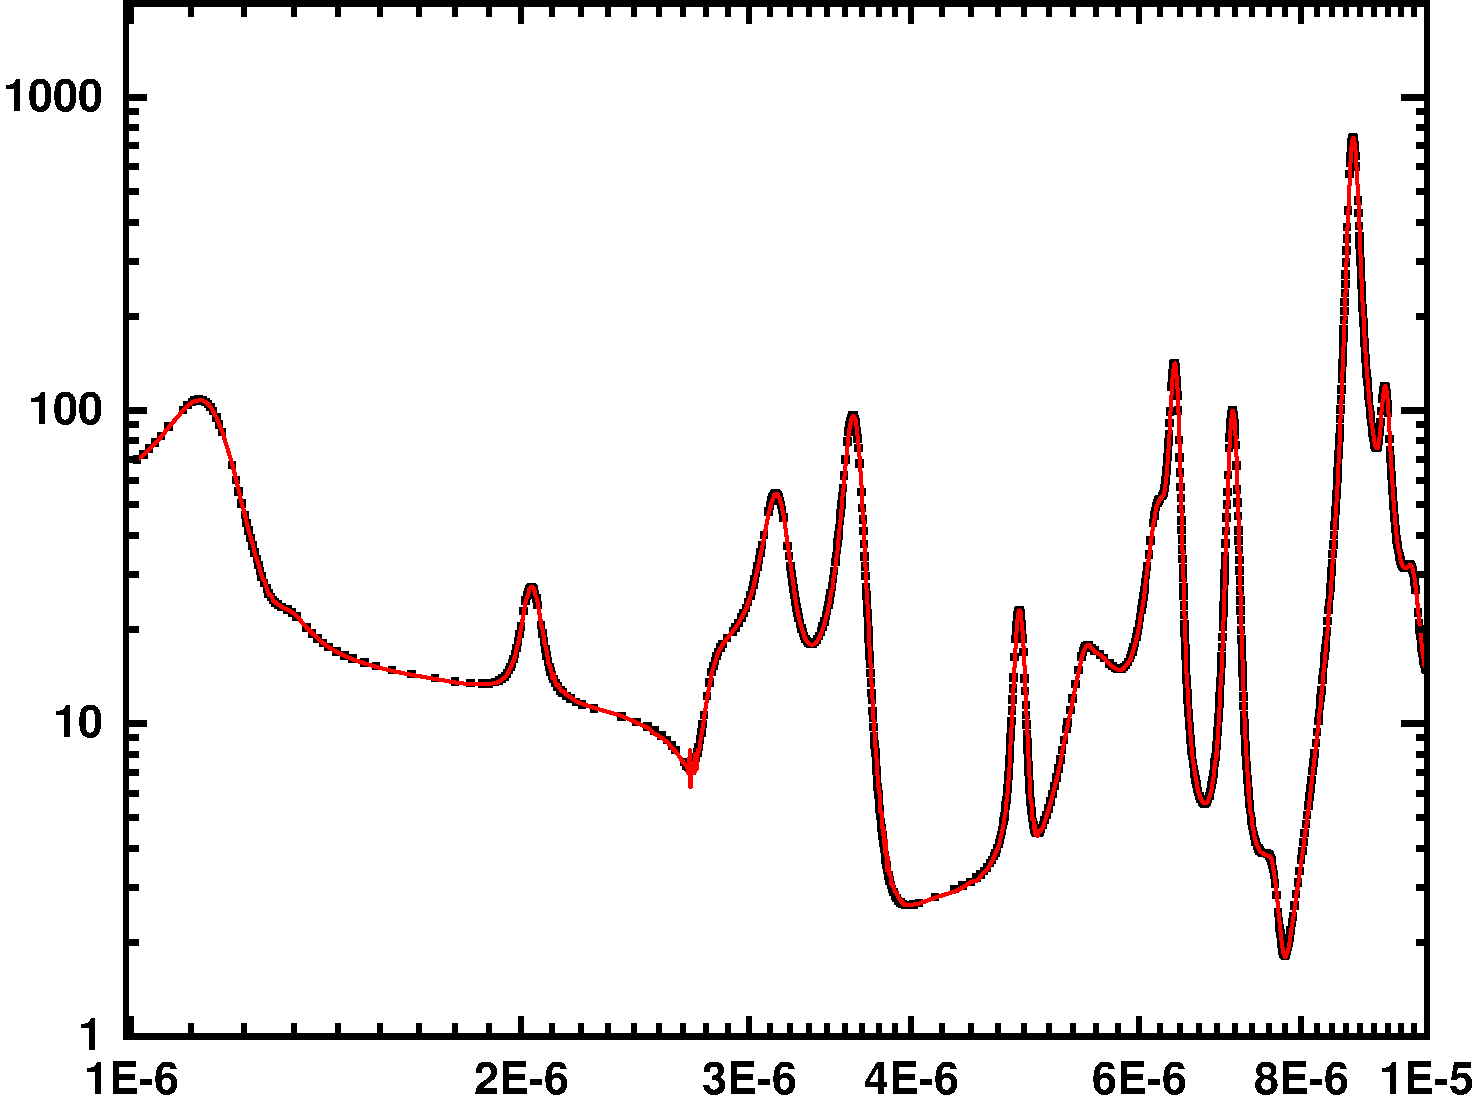
\includegraphics[width=0.84\linewidth]{figures/endftrain/G6.pdf}
  \caption{PPSDNN方法在能量区间为$[10^{-6},10^{-5}]$MeV的学习结果}
  \label{endf6}
\end{figure}
\begin{figure}[htbp!]
  \centering
  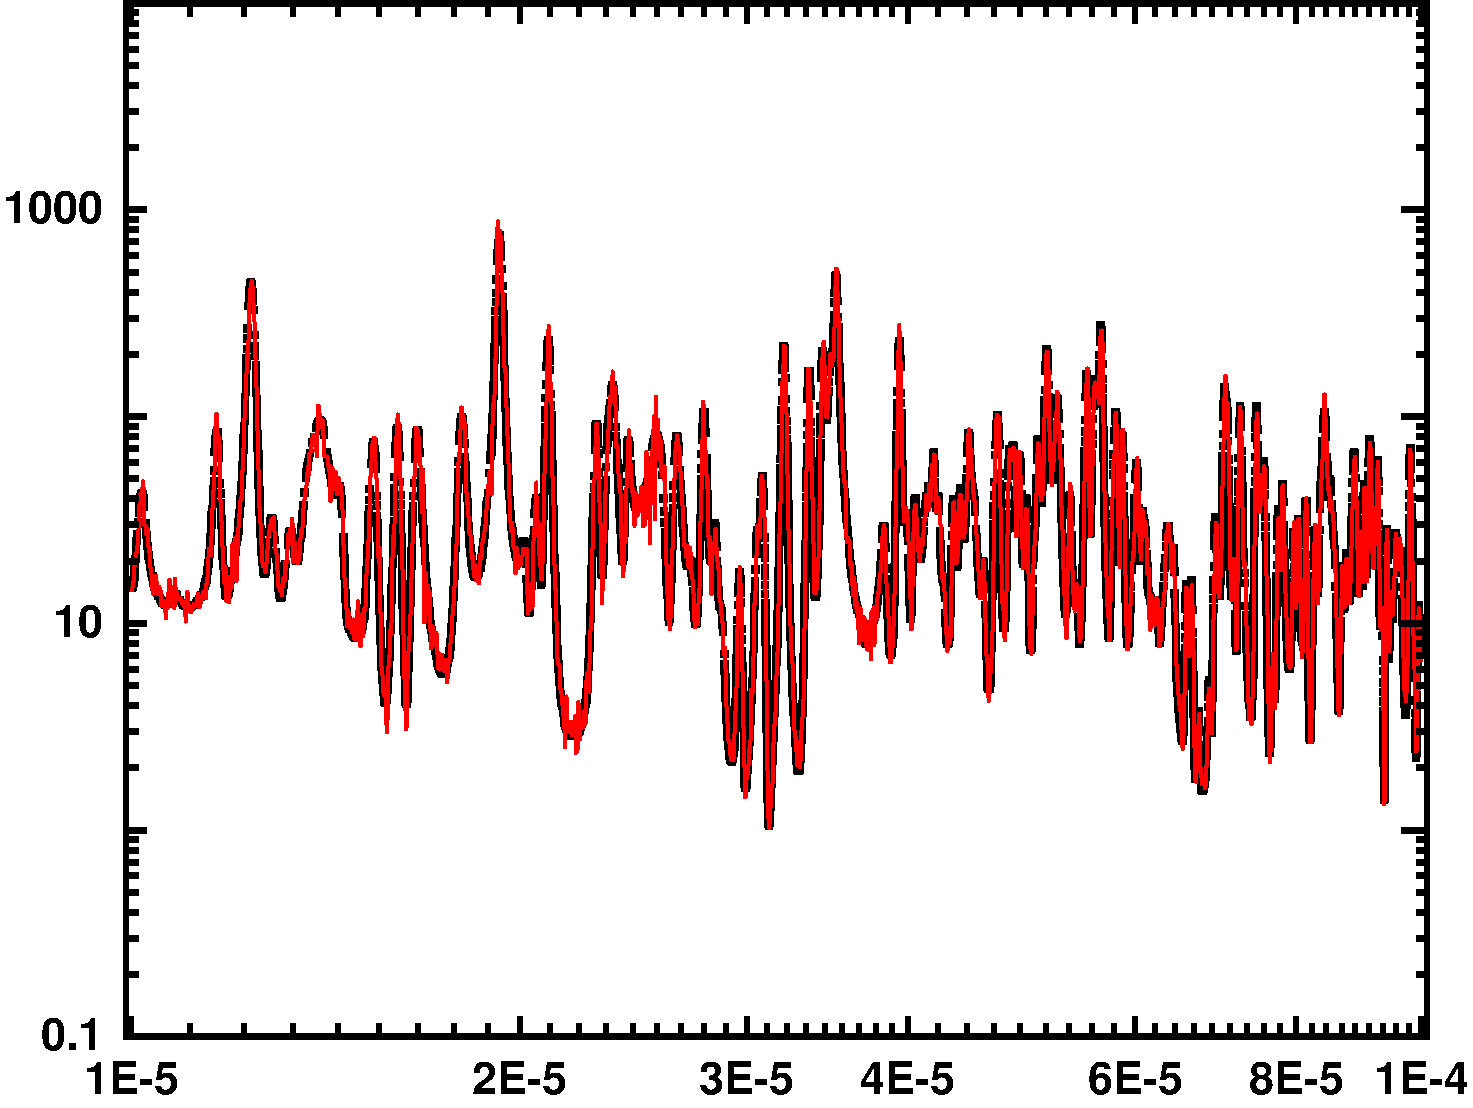
\includegraphics[width=0.84\linewidth]{figures/endftrain/G5.pdf}
  \caption{PPSDNN方法在能量区间为$[10^{-5},10^{-4}]$MeV的学习结果}
  \label{endf5}
\end{figure}
\begin{figure}[htbp!]
  \centering
  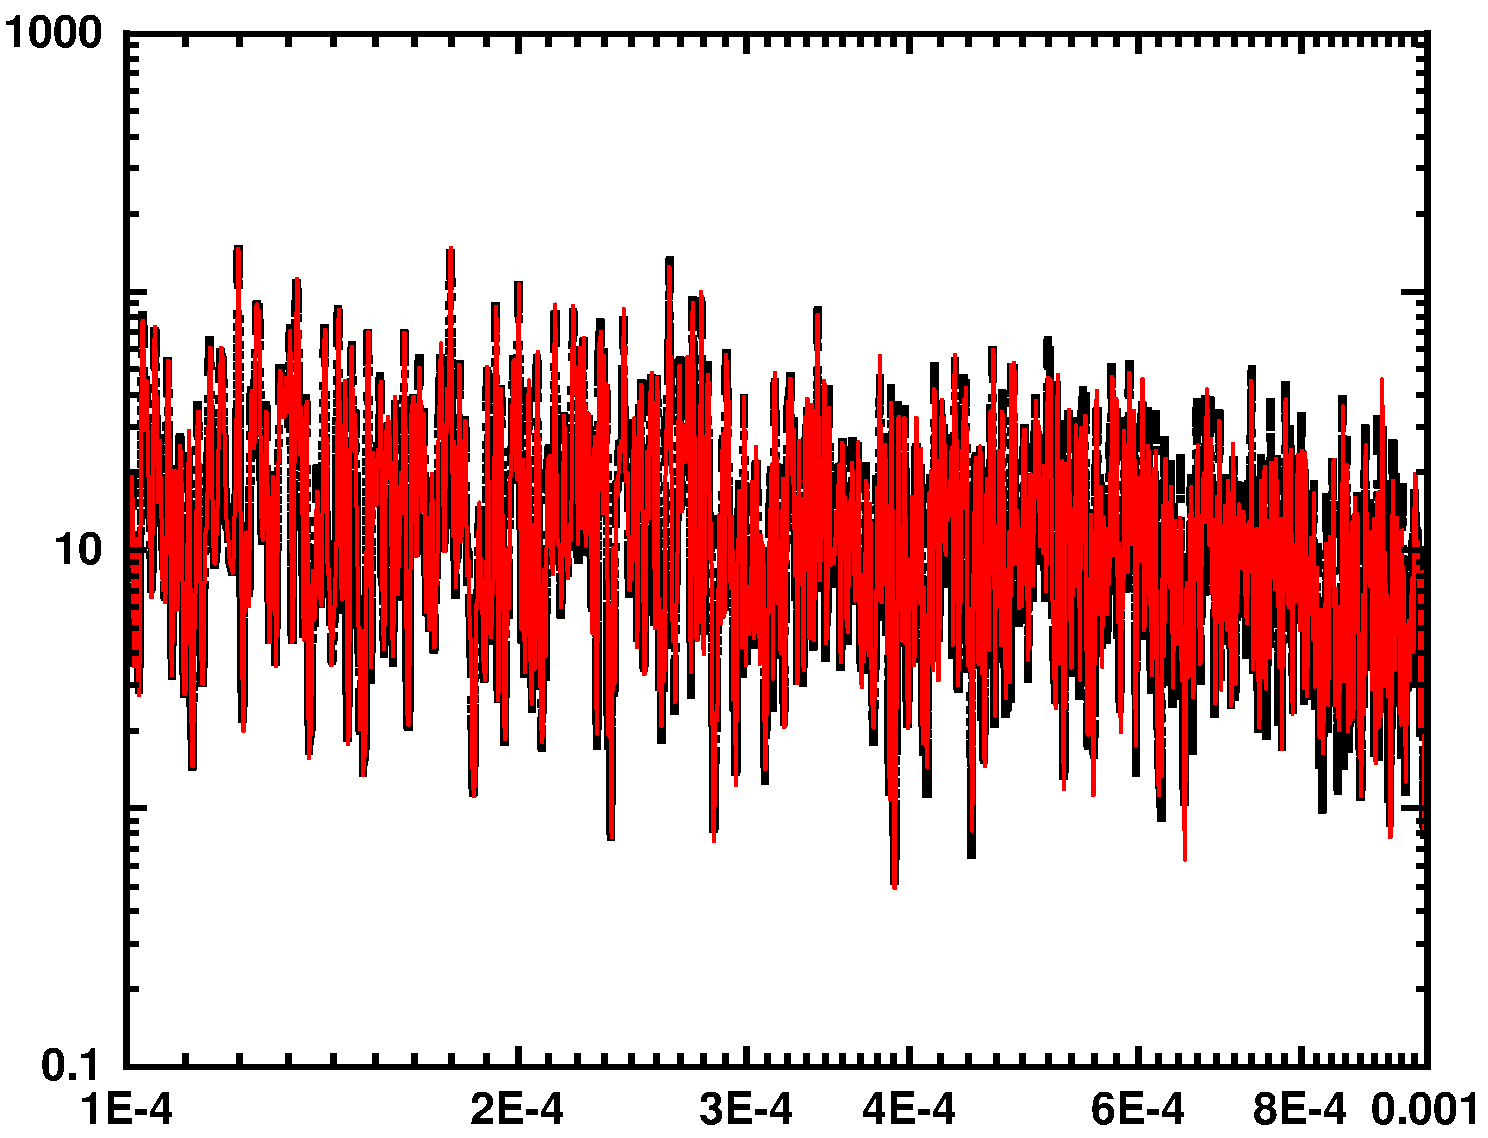
\includegraphics[width=0.84\linewidth]{figures/endftrain/G4.pdf}
  \caption{PPSDNN方法在能量区间为$[10^{-4},10^{-3}]$MeV的学习结果}
  \label{endf4}
\end{figure}
\begin{figure}[htbp!]
  \centering
  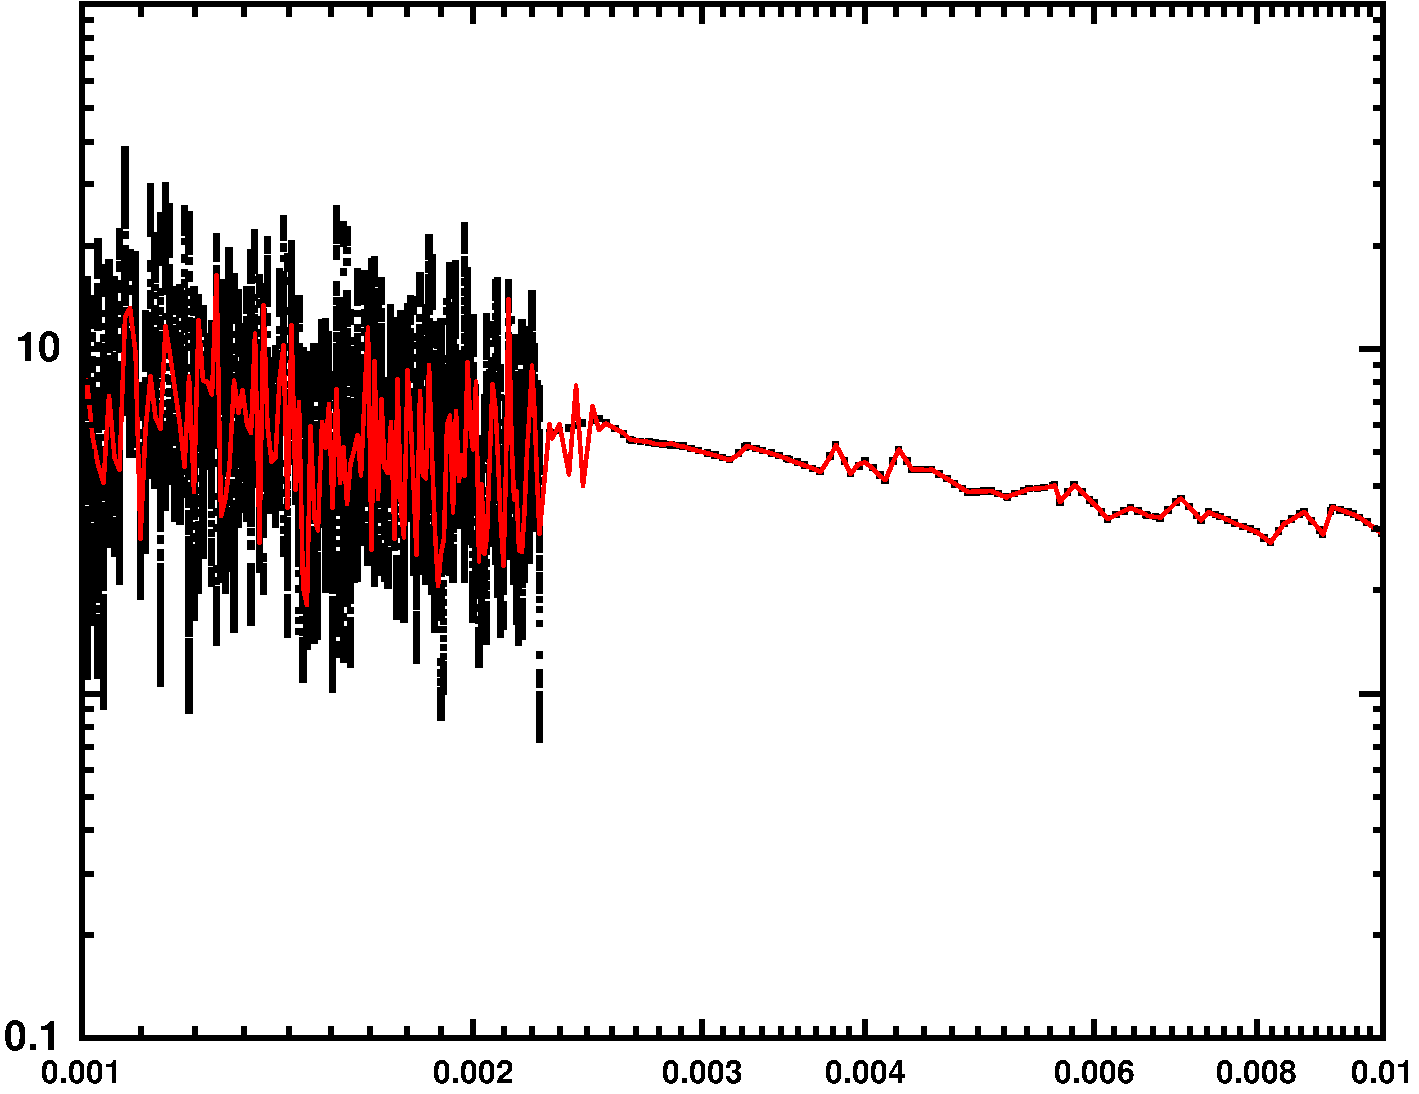
\includegraphics[width=0.84\linewidth]{figures/endftrain/G3.pdf}
  \caption{PPSDNN方法在能量区间为$[10^{-3},10^{-2}]$MeV的学习结果}
  \label{endf3}
\end{figure}
从图中可以看出,PPSDNN可以较好地学习到入射能为$10^{-6}\thicksim 0.001$MeV共振区的评价库数据。当入射能超过0.001MeV时,可以用来学习的数据量大大减少,且接近不可分辨共振区,因此会在一小段能区无法重现评价库数据。当能量大于0.003MeV时,PPSDNN可以学习到不可分辨共振区的数据。

由于评价库的核数据和实验数据相比更具有光滑性,而我们的目的是根据实验数据给出一套自己的核数据评价方法。因此后续将尝试使用PPSDNN方法直接学习$^{235}\text{U}(n,f)$反应截面的实验数据。
\begin{figure}[htbp!]
  \centering
  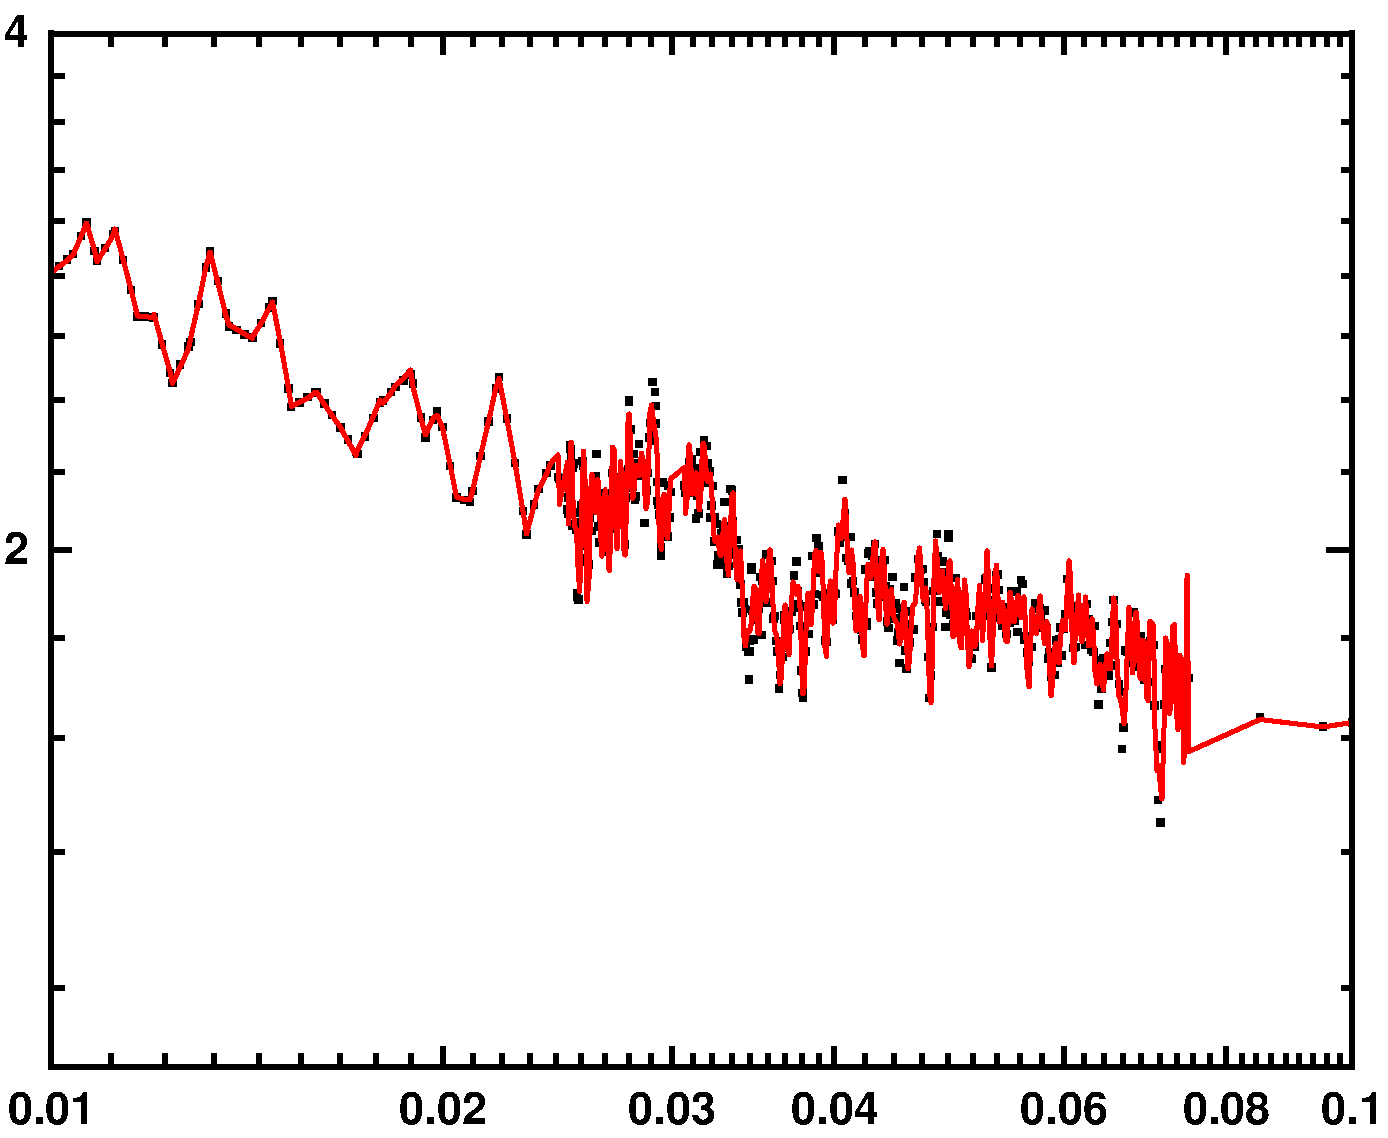
\includegraphics[width=0.63\linewidth]{figures/endftrain/G2.pdf}
  \caption{PPSDNN方法在能量区间为$[10^{-2},10^{-1}]$MeV的学习结果}
  \label{endf2}
\end{figure}
\begin{figure}[htbp!]
  \centering
  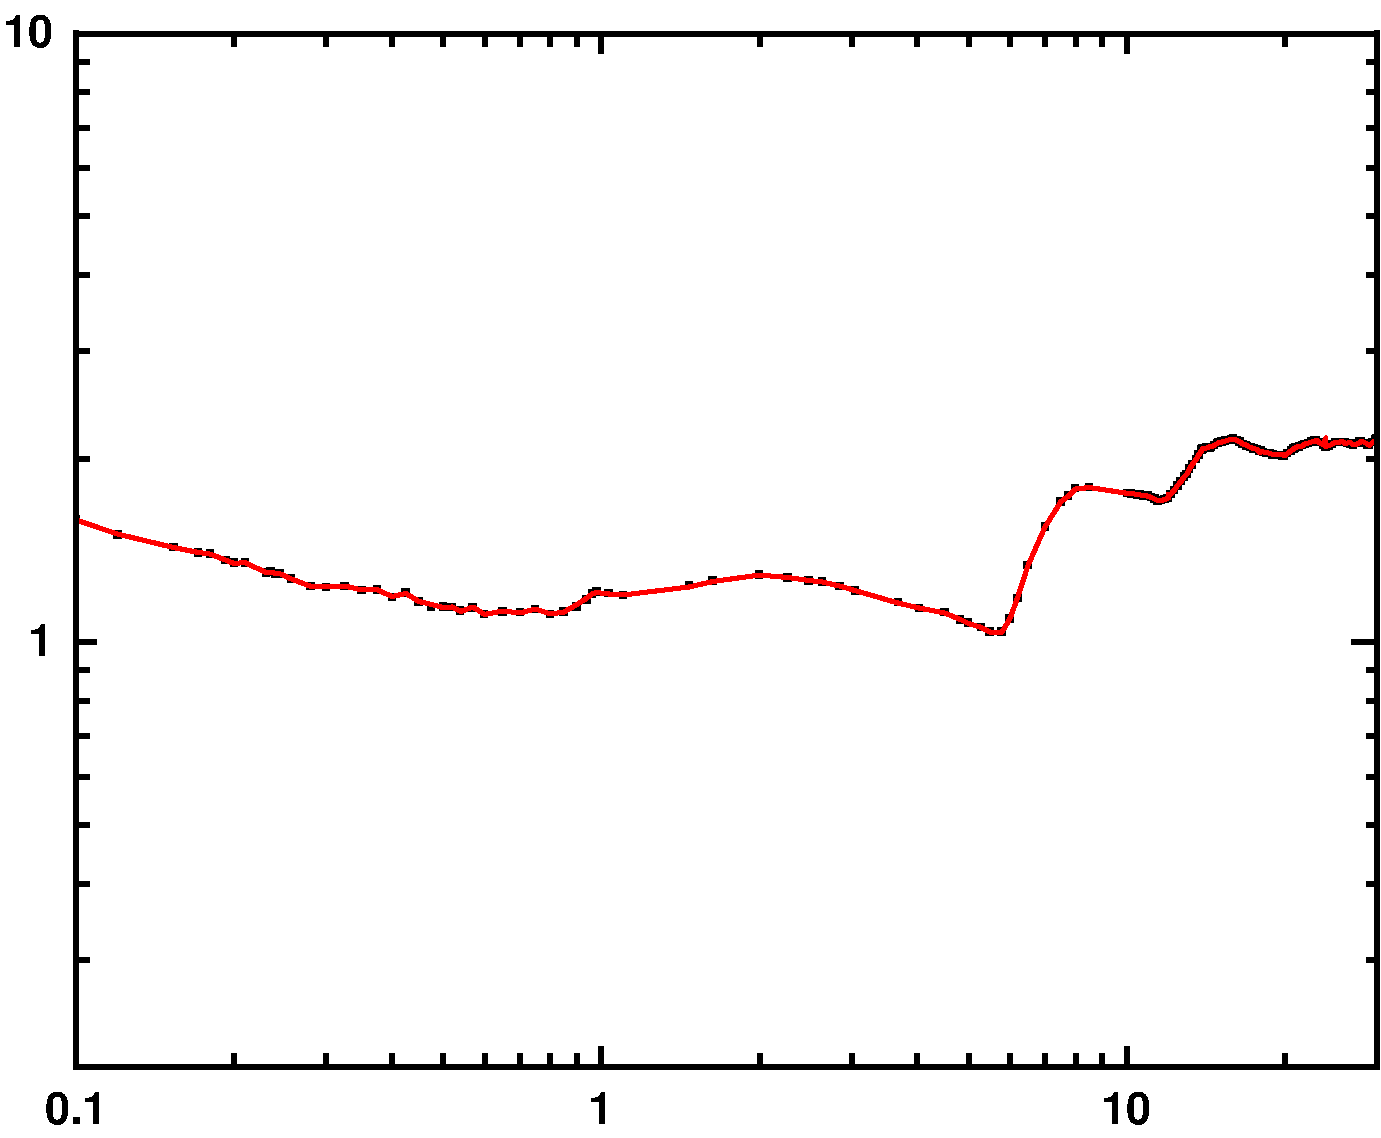
\includegraphics[width=0.63\linewidth]{figures/endftrain/G1.pdf}
  \caption{PPSDNN方法在能量区间为$[0.1,30]]$MeV的学习结果}
  \label{endf1}
\end{figure}




% 下面是学习结果

% 等结果跑出来ing





